\documentclass{beamer}
\usetheme{default}
\setbeamertemplate{navigation symbols}{}	
\usepackage{subfig}
\usepackage{epstopdf}
\usepackage{amsmath, amsthm, amssymb}
\usepackage{float}
\usepackage{rotating}
\usepackage{graphicx}
\usepackage{longtable}
\usepackage{xcolor}
\usepackage{bm}
\usepackage{tikz}
\usetikzlibrary{shapes}
\tikzset{My Arrow Style/.style={single arrow, fill=red!50, anchor=base, align=center,text width=.5cm,rotate =270}}
\newcommand{\MyArrow}[2][]{\tikz[baseline] \node [My Arrow Style,#1] {#2};}
\tikzset{My 2Arrow Style/.style={single arrow, fill=red!50, anchor=base, align=center,text width=.5cm,rotate =90}}
\newcommand{\MyArrowUp}[2][]{\tikz[baseline] \node [My 2Arrow Style,#1] {#2};}
\newcommand{\bmat}{\begin{matrix}}
\newcommand{\emat}{\end{matrix}}
\newcommand{\ov}{\overline}
\newcommand{\un}{\underline}
\newcommand{\EE}{\mathbb E}
\newcommand{\var}{\mathrm{var}}
\newcommand{\cov}{\mathrm{cov}}
\newcommand{\corr}{\mathrm{corr}}
\newcommand{\dd}{\displaystyle}
\newcommand{\ZZ}{\mathbb{Z}}
\newcommand{\RR}{\mathbb{R}}
\newcommand{\FF}{\mathbb F}
\newcommand{\LL}{\mathbb L}
\newcommand{\MM}{\mathbb M}
\newcommand{\KK}{\mathbb K}
\newcommand{\HH}{\mathbb H}
\newcommand{\QQ}{\mathbb Q}
\newcommand{\CC}{\mathbb{C}}
\newcommand{\Pin}{P_{\text{in}}}
\newcommand{\bx}{\mathbf{x}}
\newcommand{\bp}{\mathbf{p}}
\newcommand{\by}{\mathbf{y}}
\newcommand{\cP}{{\cal P}}
\newcommand{\bB}{\mathbf B}
\newcommand{\bM}{\mathbf M}
\newcommand{\bS}{\mathbf S}
\newcommand{\phis}{\varphi}
\newcommand{\barphis}{\overline\phis}
\newcommand{\se}{\text{se}}
\newcommand{\daga}{a^\dagger}
\newcommand{\devides}{\bigl |}
\newcommand{\eval}{\biggl |}
\newcommand{\ybar}{\overline y}
\newcommand{\bWhat}{\hat{\mathbf W}}
\newcommand{\bW}{\mathbf W}
\newcommand{\bz}{\mathbf z}
\newcommand{\bs}{\mathbf s}
\newcommand{\rightas}{\stackrel{a.s.}{\rightarrow}}
\newcommand{\rightp}{\stackrel{p}{\rightarrow}}
\newcommand{\rightd}{\stackrel{d}{\rightarrow}}
\newcommand{\bI}{\mathbf I}
\newcommand{\barB}{{\overline B}}
\newcommand{\barC}{{\overline C}}
\newcommand{\pbar}{{\overline p}}
\newcommand{\bbar}{{\overline b}}
\newcommand{\mubar}{{\overline \mu}}
\newtheorem{acknowledgement}[theorem]{Acknowledgement}
\newtheorem{algorithm}[theorem]{Algorithm}
\newtheorem{assumption}{Assumption}
\newtheorem{axiom}{Axiom}
\newtheorem{case}[theorem]{Case}
\newtheorem{claim}[theorem]{Claim}
\newtheorem{conclusion}[theorem]{Conclusion}
\newtheorem{condition}[theorem]{Condition}
\newtheorem{conjecture}{Conjecture}
\newtheorem{criterion}[theorem]{Criterion}
\newtheorem{proposition}{Proposition}
\newtheorem{summary}[theorem]{Summary}
\newtheorem{exercise}{Exercise}
\newtheorem{notation}{Notation}
\newtheorem{remark}{Remark}
%\graphicspath{{graphs//}}

\title {Taxes, Debts,  and Redistribution}
\author{Anmol Bhandari, David Evans, Mikhail Golosov, Thomas J. Sargent}
% \today will show current date.
% Alternatively, you can specify a date.
%
\begin{document}
%
\begin{frame}
\titlepage

\end{frame}

\begin{frame}
\frametitle{Motivation}

\begin{itemize}
\item How costly are high levels of government debt? What determines welfare cost of debt?
\vspace{2mm}
\item Should the gov't try to reduce its initial high debt? If so, how
quickly?
\vspace{2mm}

\item How should tax rates, transfers, and government debt respond to aggregate shocks, especially if markets are incomplete?
\end{itemize}

\end{frame}

\begin{frame}
\frametitle{Motivation}

\begin{itemize}
\item Analysis with complete markets is well known:

\begin{itemize}
\vspace{2mm}

\item Smooth distortionary costs of raising revenue
\vspace{2mm}

\item Labor taxes are (approximately) constant
\vspace{2mm}

\item  Arrow securities used to finance all expenditure needs
\vspace{2mm}

\end{itemize}
\item Another extreme is where the government has a ``rich'' enough set of tax instruments.
\end{itemize}
\vspace{2mm}

\textbf{Our focus:} Markets less than fully complete and there are limits to redistribution

\end{frame}

\begin{frame}
\frametitle{Key ingredients}

\begin{itemize}
\vspace{2mm}
 \item \textbf{Heterogeneity:} Agents are heterogeneous in productivities and assets 
 \item \textbf{Instruments:} A tax system that is linear in labor income and an intercept that is uniform across agents
 \vspace{2mm}
 \item \textbf{Markets:}  All agents trade a \emph{single} security whose payoff might depend on aggregate shocks
\end{itemize}

\emph{Characterize optimal tax rate, transfers and asset purchases}

\end{frame}

\begin{frame}
\frametitle{US taxes: Affine taxes}
{
  \begin{figure}
    \centering
    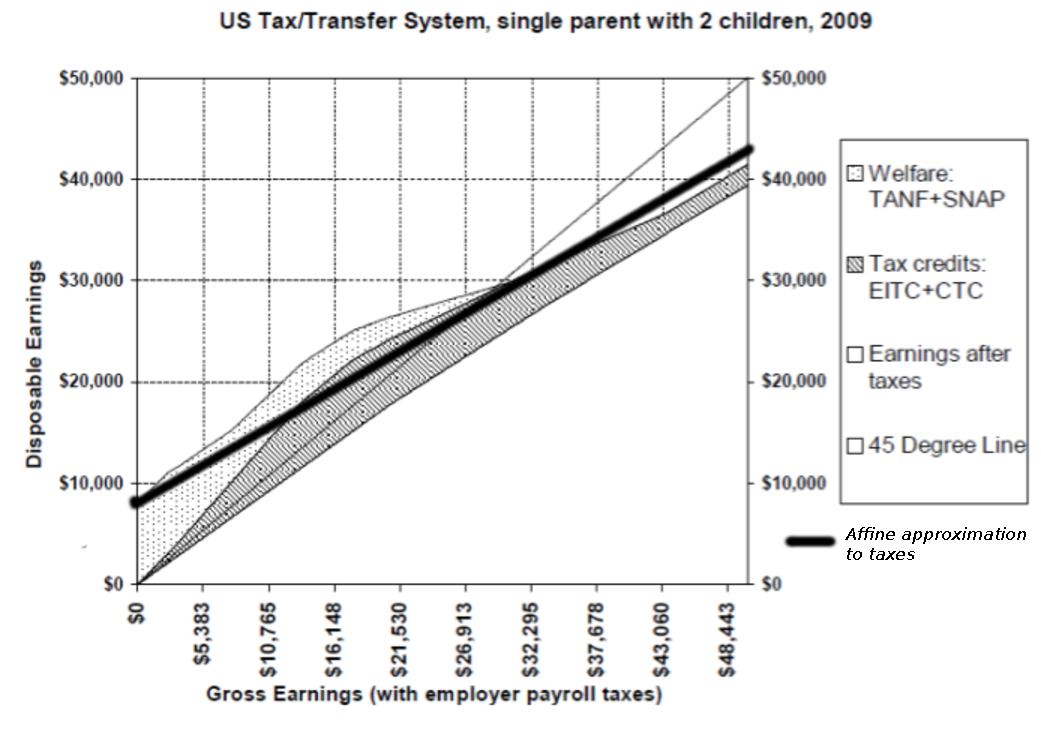
\includegraphics[width = 0.9\textwidth]{affine_taxes.pdf}
  \end{figure}

}
\end{frame}

\begin{frame}%
%EndExpansion

\frametitle{Findings I}

\begin{itemize}
\item \textbf{Welfare cost} of debt is determined by distribution of asset positions across agents

\begin{itemize}
\item Ricardian logic: Increasing all agents' assets and reducing transfers keeps budget sets unaltered
\item Costs are lower when debt is more equally distributed
\item Credit constraints (if present) may weakly improve welfare
\end{itemize}

\item \textbf{Ergodic distribution} of debts and taxes, in particular mean, variance and speed of convergence depend on

\begin{itemize}
\item \textbf{Spanning ability:} correlation of returns on the traded asset with govt's needs for revenue, and 
\item \textbf{Redistribution concerns:} Welfare weights relative to ``market'' weights that depend on wealth and productivities
\end{itemize}


\end{itemize}


\end{frame}%

\begin{frame}%
\frametitle{Findings II}
\begin{itemize}

\item What mechanisms drives \textbf{long run debt and tax rates}?

\begin{itemize}

\item If interest rate co-moves with revenue needs: issue positive debt

\item Larger the correlation: lower the magnitude debt and higher is the speed of convergence

\item More redistributive governments: larger transfers and less incentives to accumulate assets
\end{itemize}



\item  Analytical results for quasilinear preferences and some extensions to more general preferences
\end{itemize}

\end{frame}



\begin{frame}%
\frametitle{Findings III}
\begin{itemize}
\item \textbf{Calibration:} In the US data,
\begin{itemize}
\item Correlation of interest rates and business cycles is small 
\item In recent recessions, low income agents faced much larger drops in income than high income agents
\end{itemize}

\item \textbf{Optimal responses over business cycle}
\begin{itemize}
\item For short run responses, nature of shock matters
\item  In recessions with high inequality:
big increase in transfers and debt, moderate increase in tax rates
\item Normative predictions are very different from representative agent RBC models
\end{itemize}
\end{itemize}
\end{frame}

%EndExpansion

\begin{frame}%

\frametitle{Related literature}

\begin{itemize}
\item Representative agent incomplete market economies

\begin{itemize}
\item Barro (1974, 1979), Aiyagari et al (2002), Faraglia-Marcet-Scott
(2012), Farhi (2010), etc
\end{itemize}

\item Representative agent complete market economies

\begin{itemize}
\item Lucas-Stokey (1983), Chari-Kehoe (1999), etc
\end{itemize}

\item Heterogeneous agents with complete markets

\begin{itemize}
\item Werning (2007), Azzimonti-Francisco-Krusell (2008)
\end{itemize}
\end{itemize}

%TCIMACRO{\TeXButton{EndFrame}{\end{frame}}}%
%BeginExpansion
\end{frame}%
%EndExpansion







\begin{frame}
 \frametitle{Environment}
 \begin{itemize}
 \item \textbf{Uncertainty}: Markov aggregate shocks $s_t$
  \item \textbf{Demography}: N  types of infinitely lived agents (mass $n_i$)  plus a benevolent planner
  \item \textbf{Technology}: Output $\sum_{i}n_i \theta_{i,t} l_{i,t}$ is linear in labor supplies.
  \item \textbf{Preferences }(Households)
  \begin{equation*}
\mathbb{E}_{0}\sum_{t=0}^{\infty } \beta^t U^{i}\left(
c_{i,t},l_{i,t}\right)  \label{utility lifetime}
\end{equation*}%
\item \textbf{Preferences} (Planner): Given Pareto weights $\{\omega_i\}$
\begin{equation*}
\mathbb{E}_{0}\sum_{i} \omega_i\sum_{t=0}^{\infty }\beta^t U_{t}^{i}\left( c_{i,t},l_{i,t}\right)  \label{govmt objective}
\end{equation*}
  \item \textbf{Asset markets}: A risky bond with payoffs $P_t=\mathbb{P}(s_t|s_{t-1})$
  \end{itemize}

\end{frame}



\begin{frame}
 \frametitle{Environment, II}
 \begin{itemize}
  \item \textbf{Affine Taxes}: Agent $i$'s tax bill
\[- T_t + \tau_t \theta_{i,t}l_{i,t}\]

\item[]
  \item \textbf{Budget constraints} Let $R_{t-1,t}=\frac{P_t}{q_{t-1}}$
  \begin{itemize}
   \item Agent $i$: $ c_{i,t}+b_{i,t}=\left( 1-\tau _{t}\right) \theta _{i,t}l_{i,t}+R_{t-1,t}b_{i,t-1}+T_{t}$
\item Government: $g_{t}+B_{t}+T_t=\tau _{t}\sum_i n_i \theta_{i,t}l_{i,t}+R_{t-1,t}B_{t-1}$
  \end{itemize}

\item[]
  \item \textbf{Market Clearing}
  \begin{itemize}
   \item Goods: $\sum_{i}n_ic_{i,t}+g_t =\sum_i n_i \theta _{i,t} l_{i,t}$

   \item Assets: $\sum_{i}n_ib_{i,t} +B_{t}=0$

  \end{itemize}
  \item[]

\item \textbf{Initial conditions}:  $(\{b_{i,-1},B_{-1}\}_i,s_{-1})$
\end{itemize}
\end{frame}



\begin{frame}
 \frametitle{Ramsey Problem}
\label{ramsey-problem}
\begin{definition}
\textbf{Allocation, price system, government policy}: Standard

\end{definition}

\begin{definition}
\textbf{Competitive equilibrium}: Given $\left(\{b_{i,-1}\}_i,B_{-1},s_{-1}\right) $ and $\left\{ \tau _{t},T_{t}\right\} _{t=0}^{\infty }$, a competitive equilibrium is an allocation and price system such that households are optimizing and markets clear 
\end{definition}

\begin{definition}
\textbf{Optimal competitive equilibrium}: A welfare-maximizing competitive
equilibrium for a given $\left( \{b_{i,-1}\}_i,B_{-1},s_{-1}\right) $
\end{definition}
 \end{frame}



 \begin{frame}
  \frametitle{Ricardian Equivalence}
\emph{Result}: A \textbf{large set} of transfers and asset profiles support the same competitive equilibrium allocation

\textbf{Notation}: $\tilde{b}_{i,t}=b_{i,t}-b_{1,t}$: \textbf{relative assets} of Agent $i$
  \small
 \begin{theorem}
 Given $\left( \left \{ b_{i,-1}\right \} _{i},B_{-1}\right) $,let $\left \{ \left \{ \color{red}{c}_{i,t},l_{i,t},\color{black}b_{i,t}\right \} _{i},B_{t},\color{red}{R}_{t}\color{black}\right \} _{t} $ and $\left \{ \color{red}\tau _{t}\color{black},T_{t}\right\} _{t}$ be a competitive equilibrium.

 For any bounded sequences $\left \{ \hat{b}_{i,t}\right \} _{i,t\geq -1}$ that satisfy
 \begin{equation*}
 \hat{b}_{i,t}-\hat{b}_{1,t}=\tilde{b}_{i,t}\text{ for all }t\geq -1,i\geq 2,
 \end{equation*}%
 there exist  sequences $\left \{ \hat{T}_{t}\right \} _{t}$ and $%
 \left \{ \hat{B}_{t}\right \} _{t\geq -1}$ such that $\left \{ \left \{ \color{red}{c}_{i,t},l_{i,t}\color{black},\hat{b}%
 _{i,t}\right \} _{i},\hat{B}_{t},\color{red}{R}_{t}\color{black}\right \} _{t}$ and $\left \{
 \color{red}{\tau}_{t}\color{black},\hat{T}_{t}\right \} _{t}$ constitute a competitive
 equilibrium given $\left( \left \{ \hat{b}_{i,-1}\right \} _{i},\hat{B}%
 _{-1}\right) $.
 \end{theorem}
\end{frame}

\begin{frame}\label{ricardian eqv}
 \frametitle{Ricardian Equivalence: Implications}
 \begin{itemize}
\item Present value of tax revenues and gov't debt is pinned down but not period-by-period transfers

\item Can set $b_{i,t}=0$ for any $t,$ $i$ or government without loss of
generality

 \item Generally, more equally spread debt promised (implicit Social Security
promises, debt in Japan) are less distortionary than debt skewed towards
highly productive agents or foreigners (debt in Greece)

 \item \textbf{Extension:} Welfare is weakly higher with exogenous borrowing constraints of the form $b_{i,t}>\underline{b}_i$ 

\hyperlink{credit limits}{\beamerbutton{More details}}

\end{itemize}
\end{frame}


\begin{frame}
\frametitle{Characterization of optimal policy: Road map}
\begin{itemize}
\item Active channels:
\begin{enumerate}
\item Limited hedging ability
\item Concerns for redistribution
\end{enumerate}
\item Analytical results:
\begin{enumerate}
\item Quasi Linear preferences :$u(c,l)=c-\frac{l^{1+\gamma }}{1+\gamma }$
\item IID aggregate shocks
\end{enumerate}
\item 2 step build up:
\begin{enumerate}
\item Assume first that there is one agent and no ability to use $T$
\item Use results to characterize outcomes in the more general settings with heterogeneous agents and no restriction on transfers
\item Allows us to disentangle hedging and redistribution motives
\item Informative about the setup with multiple agents where transfers are unrestricted but their costs are endogenously high
\end{enumerate}
\end{itemize}
\end{frame}

\begin{frame}%
%EndExpansion
\frametitle{Single agent quasi-linear economy with $T\equiv 0$}

Let $V(B\_)$ be the maximum ex-ante value the government can achieve with assets $B\_$. 

\[V(B\_)=\max_{c(s),l(s),B(s)} \sum_{s}\pi(s)\left\{c(s)-\frac{l(s)^{1+\gamma}}{1+\gamma}+\beta V(B(s)) \right\}\]
subject to
\[   c(s)-B(s)=l(s)^{1+\gamma}-\beta^{-1} P(s)B\_\]
\[c(s)+g(s)\leq\theta l(s)\]

\[\underline{B}\leq B(s)\leq \bar{B}\]


\end{frame}

\begin{frame}
\frametitle{Single agent quasi-linear economy with $T\equiv 0$}
\begin{itemize}
\item Decompose the set of payoffs:

\[\mathcal{P}^{\ast }=\left\{ P(s):P(s)=1+\frac{\beta }{B^{\ast }}(g(s)-%
\mathbb{E}g)\text{ for some }B^{\ast }\in \lbrack \overline{B},\underline{B}%
]\right\} \]

\item Spanning condition that supports complete market allocations

\end{itemize}



\end{frame}


\begin{frame}

\frametitle{Invariant distribution}
\begin{theorem}
\begin{enumerate}
\small

 \item Suppose $P\not \in \mathcal{P}^*$, there is an invariant distribution of government assets such that 

\[\forall \epsilon>0, \quad \Pr\{B_t<\underline{B}+\epsilon \text{ or } B_t>\overline{B}-\epsilon \quad i.o \}=1\]

\item Suppose  $P(s)-P(s')>\beta \frac{g(s)-g(s')}{\underline{B}} \quad \forall s,s'$, then for large enough government assets (or debt) there is a drift towards the interior region.  In particular the value function $V(B)$ is strictly concave and there exists $B_1<B_2$ such that

\[\mathbb{E}V'(B(s))>V'(B\_) \quad B\_>B_2 \]
and
\[\mathbb{E}V'(B(s))<V'(B\_) \quad B\_<B_1 \]

\item Suppose $P(s)\in \mathcal{P}^*$, then the  long run government assets converge to a degenerate steady state

\[\lim_tB_t=  B^*\quad a.s \quad \forall B_{-1} \]


\end{enumerate}


\end{theorem}


\end{frame}%



\begin{frame}%
%EndExpansion

\frametitle{Perfect spanning}\label{linearization}

\begin{itemize}
\item \smallskip For $P(s)\in \mathcal{P}^{\ast },$ we can
replicate complete markets perfectly asymptotically

\item Target assets%
\begin{equation*}
B^{\ast }=\beta \frac{\mathrm{var}(g(s))}{\mathrm{cov}(P(s),g(s))}
\end{equation*}

\item Tax rate is constant in long run and inversely related to $B^*$.


\item Use this to construct an approximation for the ergodic distribution of debt and taxes of an economy with $P(s)$ ``close'' enough to $\mathcal{P}^*$. In particular split $P(s)$

\[P(s)=\hat{P}(s)+P^*(s)\] where $P^*(s)\in \mathcal{P}^*$ and $\hat{P}(s)$ is orthogonal to $g(s)$. 
\hyperlink{linear appendix}{\beamerbutton{More details}}
\end{itemize}
\end{frame}%


\begin{frame}%
%EndExpansion

\frametitle{Imperfect spanning}
\begin{theorem}

The ergodic distribution of debt (under the first order approximation of dynamics near $P^*(s)$ ) has the following properties,
\begin{itemize}
 \item \textbf{Mean:} The ergodic mean is $B^*$ which corresponds to the steady state level of govt. assets of an economy with payoff vector $P^*(s)$
  
 \item \textbf{Variance:} The coefficient of variation of assets satisfies
  \[
    \frac{\sigma(B)}{\mathbb E(B)} = \sqrt\frac{\var(P(s)) - |\cov(g(s),P(s))|}{(1+|\cov(g(s),P(s))|)|\cov(g(s),P(s))|}\leq\sqrt\frac{\var(\hat{P}(s))}{\var(P^*(s))}
  \]
  \item \textbf{Convergence rate:} The speed of convergence to the ergodic distribution is
  \[
    \frac{\EE_{t-1}(B_t-B^*)}{(B_{t-1} - B^*)} = \frac1{1+|\cov(P(s),g(s))|}
  \]

\end{itemize}
  

\end{theorem}

\end{frame}%

\begin{frame}
\frametitle{Ergodic distribution} 
\begin{figure}[htp]
 \centering
 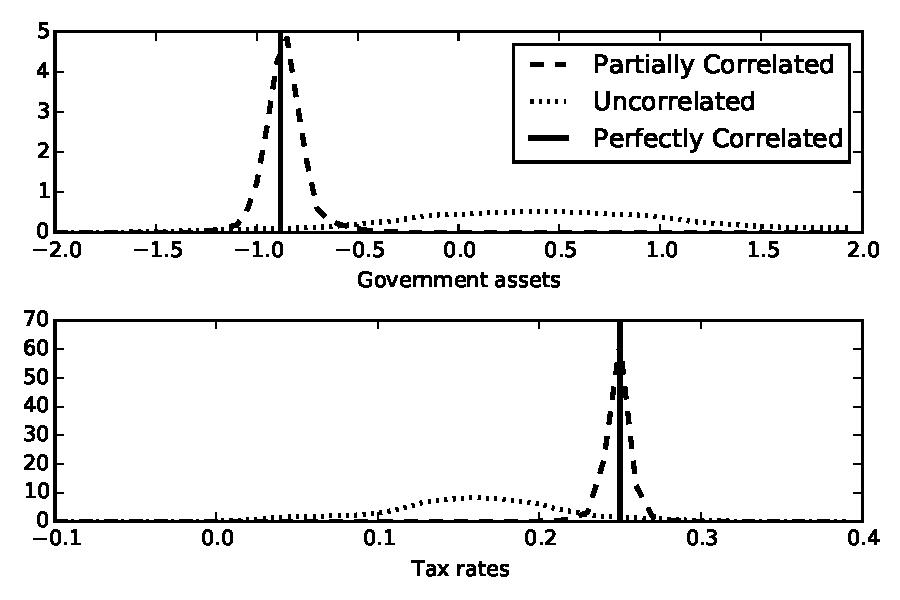
\includegraphics[width=4in]{plots/ErgodicQL.pdf}
 \caption{Ergodic distribution for debt and taxes in the representative agent quasilinear economy for three choices $P(s)$.}
 \label{fig: ergodic distribution ql}
 \end{figure}

\end{frame}


\smallskip 
%TCIMACRO{\TeXButton{BeginFrame}{\begin{frame}}}%
%BeginExpansion
\begin{frame}%
%EndExpansion

\frametitle{Summary and next steps}

\smallskip

\textbf{So far:} In a single agent - quasilinear - no transfers economy we saw that,

\begin{itemize}
\item Target level of assets maximizes spanning
\begin{itemize}
\item taxes are constant when perfect spanning is achieved
\end{itemize}
\item When markets are imperfect, can be far away from the target
\begin{itemize}
\item invariant distribution of taxes also has large support
\end{itemize}
\item Speed of moving to the target debt level depends on covariance of
asset payoff and shocks

\begin{itemize}
\item low covariance $\Longrightarrow $ slow speed
\end{itemize}
\end{itemize}

\textbf{Next:} A version with heterogeneous agents and no restrictions on transfers
\begin{itemize}
\item This adds a new instrument to hedge shocks but welfare cost of using transfers is endogenous
\item The single agent results are informative about cases where these costs are large
\end{itemize}


%TCIMACRO{\TeXButton{EndFrame}{\end{frame}}}%
%BeginExpansion
\end{frame}%
%EndExpansion

\begin{frame}
\frametitle{Heterogeneous agents}
Suppose we have 2 agents

\begin{itemize}
\item Quasi-linear preferences as before
\item Productivities: $\theta_1>\theta _{2}=0$ 
\item Pareto weights, mass of Agent 1 and 2: $\{\omega,1-\omega\}$ and $\{n,1-n\}$ respectively
\item Non-negative consumption: $c_{2}\geq 0$
\end{itemize}

Normalize $b_{2,t}=0$, thus $B_t=-nb_{1,t}$ are interpreted to be government assets
\end{frame}



\begin{frame}
\frametitle{Heterogeneous Agents}
\small
\begin{theorem}
\label{thm heterogeneous agents}
Let $\omega,n$ be the Pareto weight and mass of the productive agent with $n<\frac{\gamma}{1+\gamma}$. The optimal tax, transfer and asset policies $\{\tau_t,T_t,B_t\}$ are characterized as follows,


\begin{enumerate}
 \item For $\omega\geq n \left(\frac{1+\gamma}{\gamma}\right)$ we have  $T_t=0$ and the optimal policy is same as in our representative agent economy studied 

\item For $\omega< n \left(\frac{1+\gamma}{\gamma}\right)$, suppose we assume that  $P(s)\not \in \mathcal{P}^*$ and $\min_{s}\{P(s)\}>\beta$. There exists $\mathcal{B}(\omega)$ and $\tau^*(\omega)$ with $\mathcal{B}'(\omega)>0$ such that 

\begin{enumerate}
  \item $B\_>\mathcal{B(\omega)}$
\[T_t>0, \quad \tau_t=\tau^*(\omega), \textit{ and } B_t=B\_ \quad \forall t\] 
\item $B\_\leq \mathcal{B(\omega)}$ 
   \[T_t>0 \text{ i.o.},\quad \lim_t\tau_t=\tau^*(\omega) \text{ and } \lim_tB_t=\mathcal{B}(\omega)\quad \textit{a.s}\]
 \end{enumerate}

 \end{enumerate}

\end{theorem}

\end{frame}




\begin{frame}
\frametitle{Concerns for redistribution}

\begin{itemize}
\item Balancing costs of fluctuations in tax rates and transfer

\begin{itemize}
\item fluctuations in taxes is costly: deadweight loss

\item fluctuations in transfers is costly: deviations from target level of
redistribution
\end{itemize}

\item For large $\omega$ transfers are costly as the planner gives resources to unproductive agents 

\item For low $\omega$, transfers are used: 
\begin{itemize}
\item For low initial debt, interior solution: All shocks hedged by transfers
\item For high debt, accumulate assets until costs of transfers are equalized to costs of collecting labor taxes
\end{itemize}

\item The more redistributory the planner is:

\begin{itemize}
\item bigger average tax rates and transfers
\item less need to accumulate assets for precautionary reasons
\end{itemize}
\end{itemize}

\end{frame}



\begin{frame}
\frametitle{Risk aversion}\label{risk aversion}

\begin{itemize}
\item With risk aversion: for a (generic) set of parameters there is asset allocation replicating complete market economy

\begin{itemize}
\item arguments harder since "real"\ interest rates $\mathbb{E}_{t}U^{\prime
}\left( c_{t+1}\right) R\left( s_{t+1}\right) /U^{\prime }\left(
c_{t}\right) $ is endogenous
\end{itemize}

\item Same general flavor as quasi-linear economy

\begin{itemize}
\item cost of fluctuations in transfers comes from cost of fluctuation in $%
U_{c}$ $\Longleftrightarrow $ similar to multiplier on constraint $c\geq 0$
in quasi-linear case

\item If real payoffs are positively correlated with $g:$ accumulate assets

\item If real payoffs are (sufficiently) negatively correlated with $g:$
accumulate debt

\item absolute amount of asset/debt is decreasing in redistributive objective
\end{itemize}
\end{itemize}
\hyperlink{risk aversion annex}{\beamerbutton{More details}}
\end{frame}%


\begin{frame}
\frametitle{Numerical exercise}
 
Solve $N=5$ agent economy with realistic level and movements in wage dispersion across booms and recessions

\begin{itemize}
 \item Long run dynamics: Study settings that differ in covariance of interest rates and output
 \item Transient dynamics: Study outcomes in recessions that are accompanied by higher inequality
\end{itemize}

Aggregate shocks affect,
\begin{enumerate}
\item Wages: \[\log \theta_i=\epsilon [1+(.9-d(i))m]\]
 \item Payoffs: \[P=1+\chi \epsilon \]
\end{enumerate}

\end{frame}


\begin{frame}	
\frametitle{Calibrating $m$: Inequality over business cycles}


 {
  \begin{figure}
  \label{fig:fatih_picture}
    \centering
    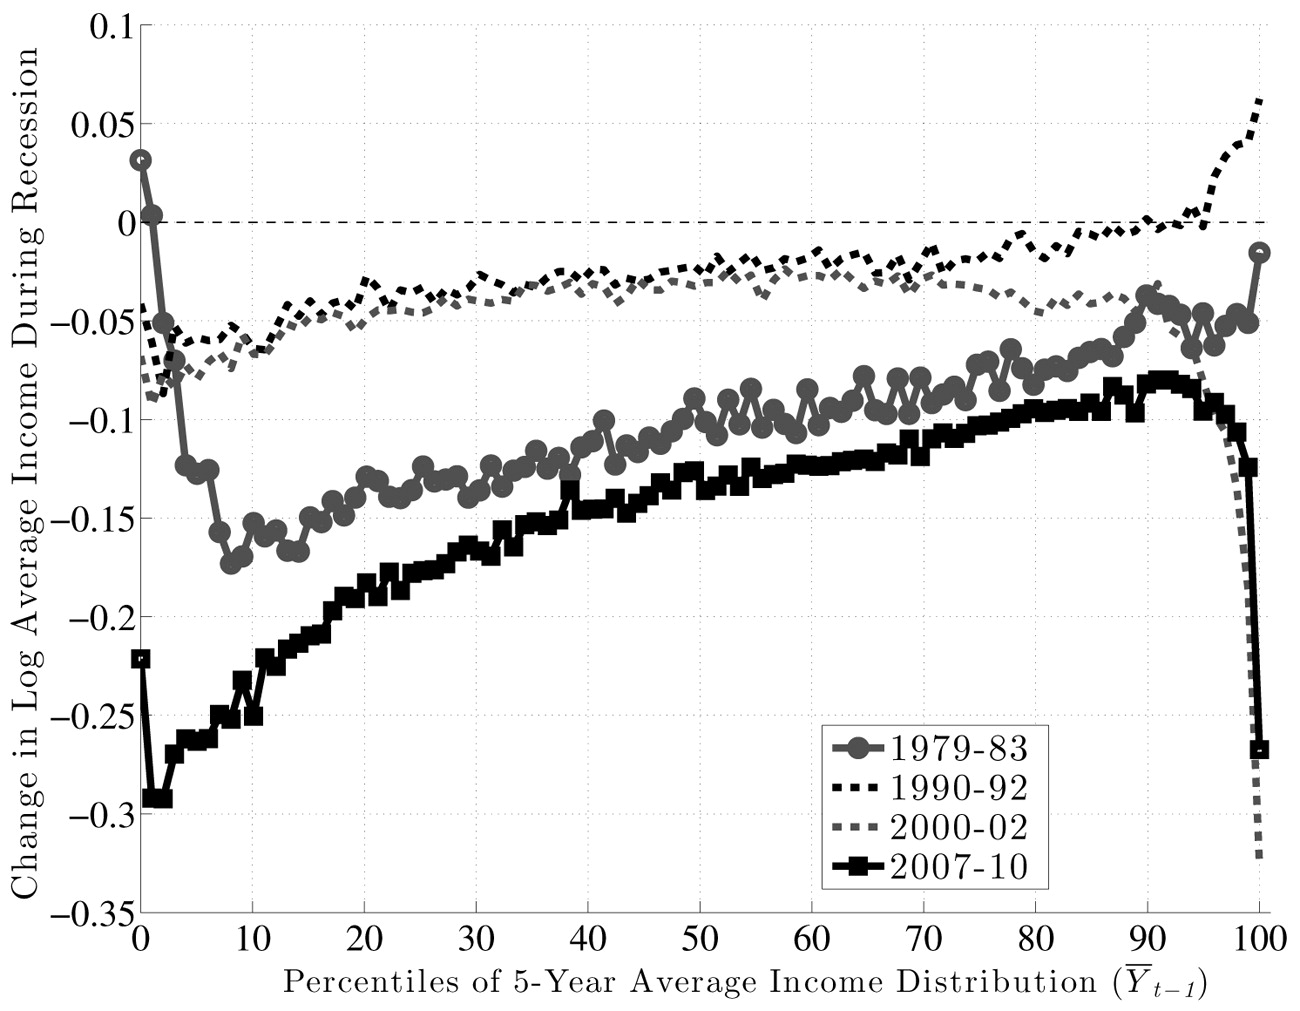
\includegraphics[width = 0.75\textwidth]{fg13.jpeg}
    \caption{ Change in log average earnings during recessions, prime-age males from Guvenen et all [2014]}
  \end{figure}

}
\end{frame}



\begin{frame}
 \frametitle{Calibrating $\chi$: Ex post variation in Payoffs}
 Let $q^{(n)}_t$ be the log price of a nominal bond of maturity $n$. We can define the real holding period returns $r^{(n)}_{t,t+1}$ as follows
 
 \[r^{(n)}_{t,t+1}= q^{(n-1)}_{t+1}-q_t^{(n)}-\pi_{t+1}\]
 With the transformation $y^{(n)}_t: -\frac{1}{n} q^{(n)}_t$ we can express $r^{(n)}_{t,t+1}$ as follows:
 \small
 \[r^{(n)}_{t,t+1}=\underbrace{y^{(n)}_t}_{\text{Ex-ante part}} - (n-1)\left[\underbrace{\left(y^{(n)}_{t+1}-y^{(n)}_{t}\right)}_{\text{Interest rate risk given $n$}}+\underbrace{\left(y^{(n-1)}_{t+1}-y^{(n)}_{t+1}\right)}_{\text{Term structure risk}}\right]-\underbrace{\pi_{t+1}}_{\text{Inflation risk}}\]
\end{frame}


\begin{frame}
 \frametitle{ Interest rates and TFP}
 \small
 \begin{itemize}
  \item In the model the holding period returns are given by $\log\left[\frac{P_{t+1}}{q^{1}_{t}}\right]$ and $q^{1}_t=\frac{\beta \mathbb{E}_tu_{c,t+1}P_{t+1}}{u_{c,t}}$. 
\item $P_{t+1}$ allows us to captures ex-post fluctuations in returns to the government's debt  portfolio coming from maturity and inflation. 
\item Since $\epsilon_{t}$ is i.i.d over time in our calibration  $\chi=\frac{\sigma_{r}}{\sigma_{\epsilon}} Corr(r,\epsilon)$
 \end{itemize}

 Using data on labor productivity $\epsilon_{t}$ and $\{q^{n}_t\}_{n}$:
 
\begin{table}[htp]
\small
\begin{tabular}{|l|l| l|l|l|}
\hline
Maturity (n) &2yr & 3yr & 4yr & 5yr\\
\hline
$Corr(\epsilon_{t+1},r^{(n)}_{t,t+1})$ & -0.11 &-0.093 &-0.083 &-0.072\\
$Corr(\epsilon_{t+1},r^{(n)}_{t,t+1}-ny^{(n)}_{t})$& 0.00 & -0.0463 &-0.080& -0.091\\
$Corr(\epsilon_{t+1},y^{(n)}_{t}-\pi_{t+1})$ &-0.097  &-0.086  &-0.080  &-0.073 \\ 
$\frac{\sigma({r^{n}_{t+1}})}{\sigma({\epsilon_{t+1}})}$  &0.820  &0.835  &0.843  &0.845\\ 

\hline
\end{tabular}
\caption{}
\label{tab:corr}
\end{table}
 
\end{frame}


\begin{frame}
\frametitle{Calibration}

\begin{table}[htp]
\tiny
\begin{tabular}{|l|c|p{4cm}|}
\hline
Parameter & Value & Description   \\ \hline
$\{\bar{\theta}_i\} $ & \{1 ,  1.4,  2.1,  3.24,  4.9\} & Wages dispersion for \{10,25,50,75,90\} percentiles   \\
$\gamma$ & 2 & Average Frisch elasticity of labor supply of 0.5 \\
$\beta$ & 0.98  &Average (annual) risk free interest rate of 2\%   \\
$m$ &$\frac{1.5}{.8}$& Changes in dispersion \\
$\chi$ & -0.06 & covariance between holding period returns and labor productivity \\
$\sigma_e$ & 0.03 & vol of labor productivity\\
$g$ & .13 \%&Average pre-transfer expenditure- output ratio of 12 \% \\\hline
\end{tabular}
\caption{Benchmark calibration}
\label{tab:Parameters}
\end{table}
\scriptsize
The Pareto weights and initial distribution of wealth are chosen to match an average tax rate of $20\%$, and debt to gdp ratio of $100\%$,  transfers to gdp ratio of 10\%,  and deciles of US wealth distribution
\end{frame}

\begin{frame}
\frametitle{Long run}
 {
  \begin{figure}
    \centering
    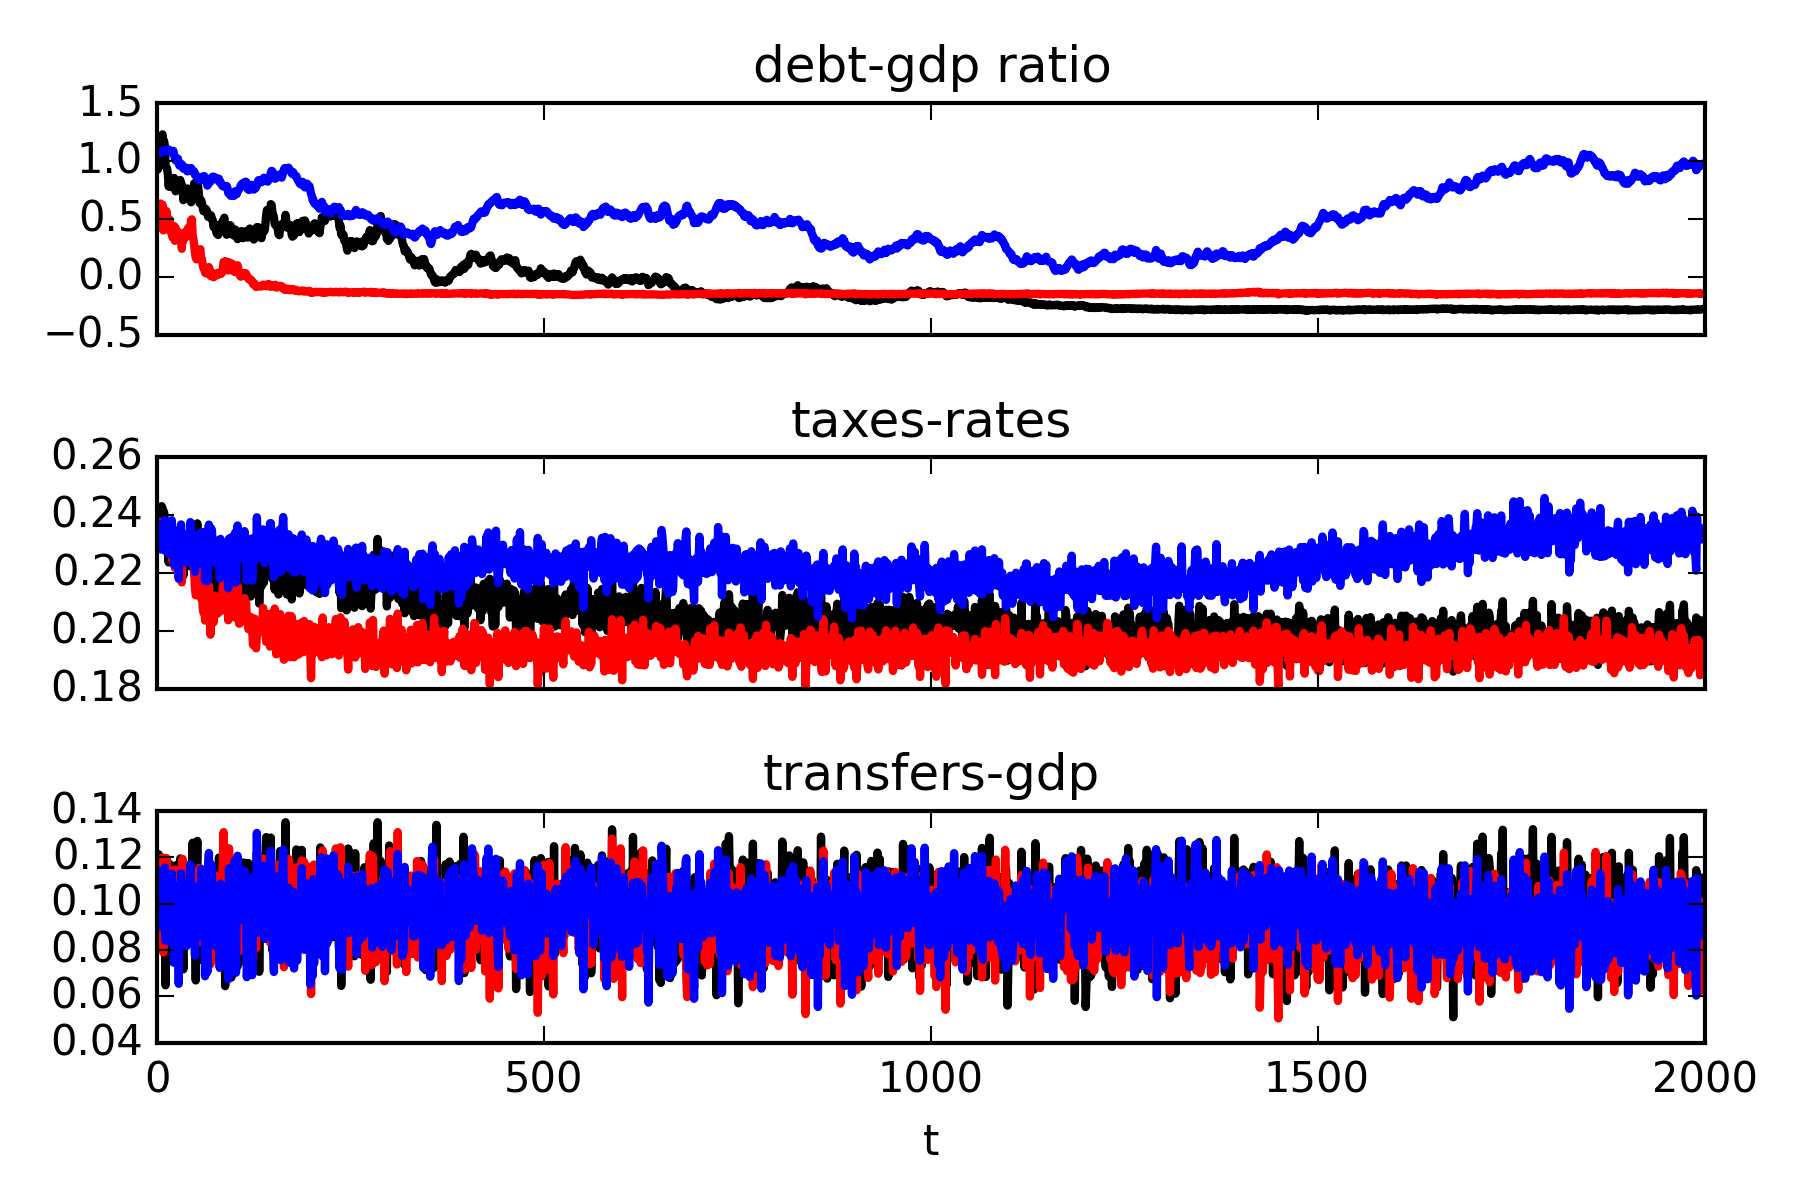
\includegraphics[width = 0.9\textwidth]{cesplots/long_simulation_debt.png}
    \caption{The red, black and blue lines plot simulations for a common sequence of shocks for values of $\chi=-1.0,0,1.0$ respectively}
  \end{figure}

}

\end{frame}


\begin{frame}
\frametitle{Long run: Speed of convergence}
 {
  \begin{figure}
    \centering
    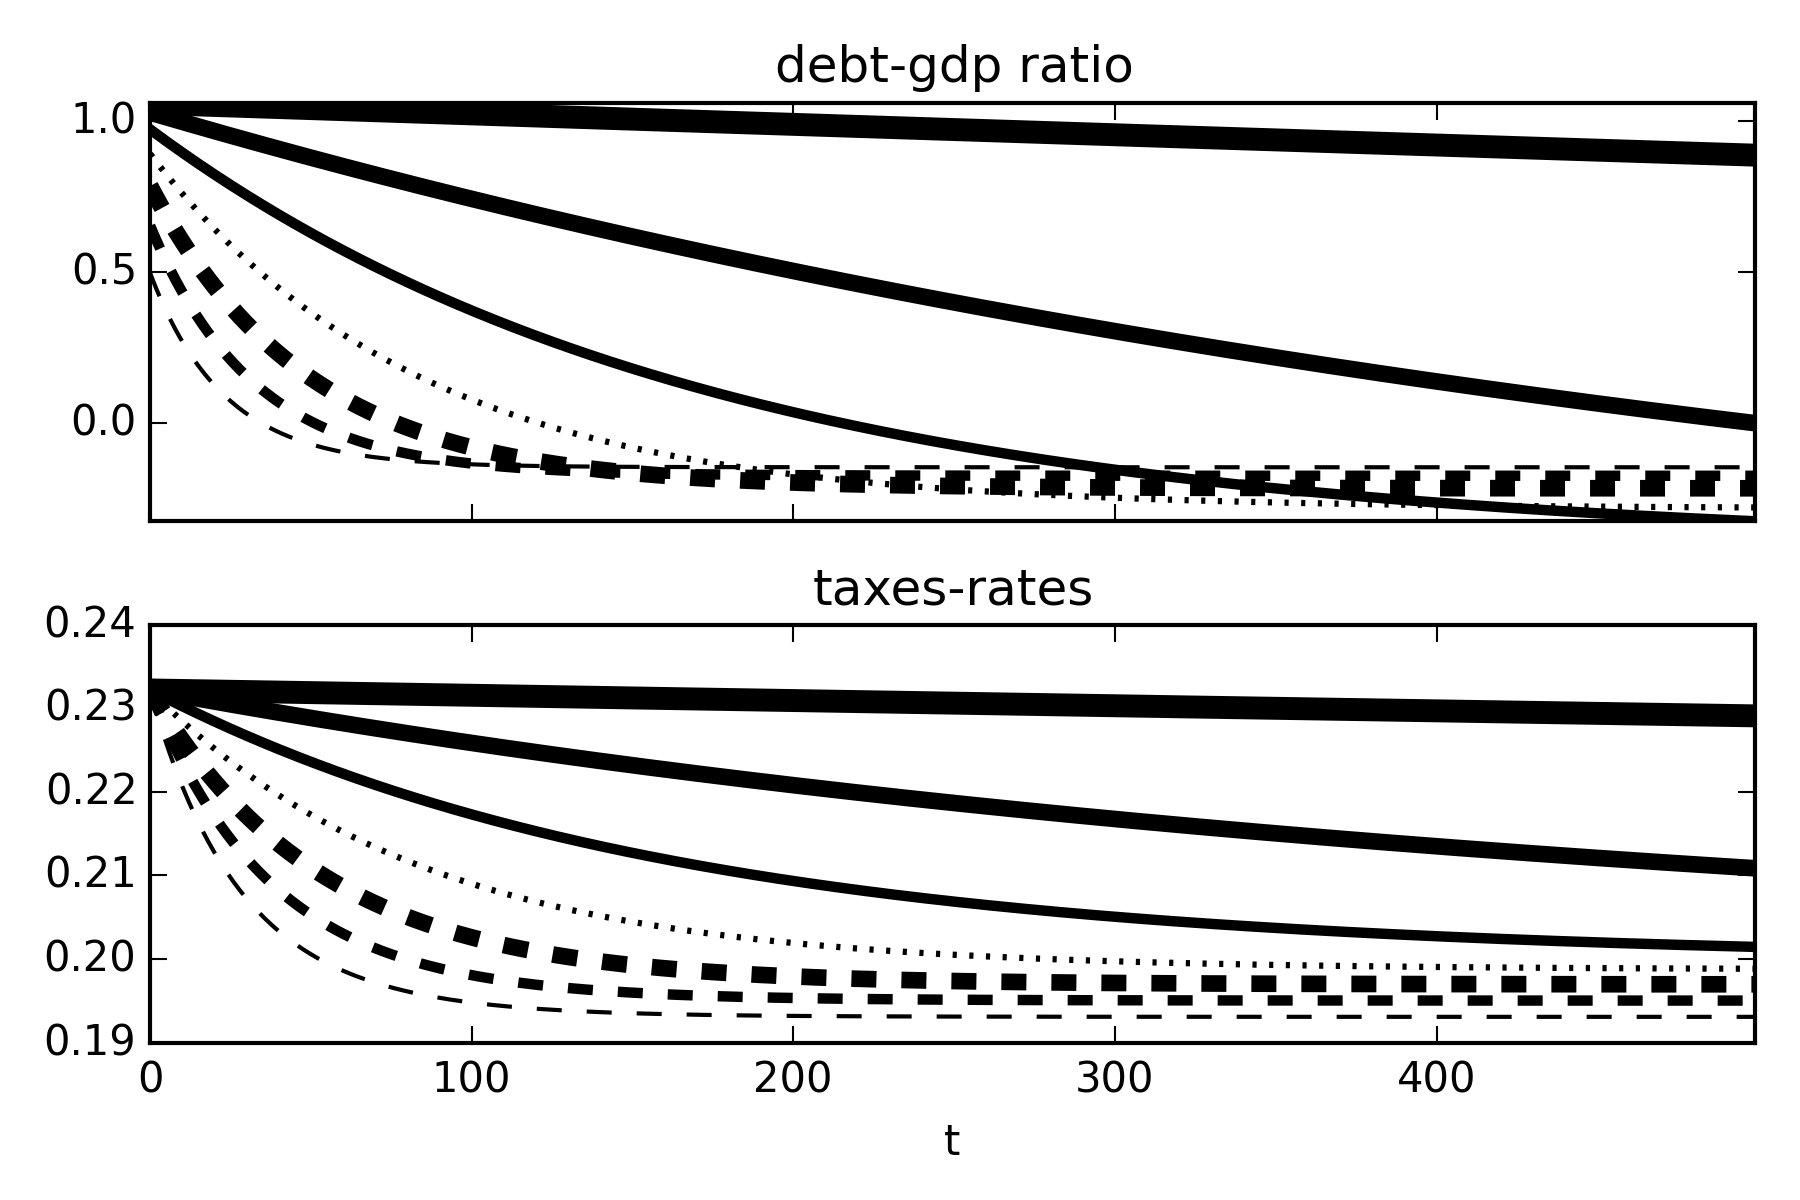
\includegraphics[width = 1.0\textwidth]{cesplots/speed_of_convergence.png}
    \caption{The plot shows conditional mean paths for different values of $\chi$. The red (blue) lines have $\chi<0$ ($\chi>0$). The thicker lines represent larger values.}
  \end{figure}

}

\end{frame}

\begin{frame}
 \frametitle{Spreading of tax rates}
{
  \begin{figure}
    \centering
    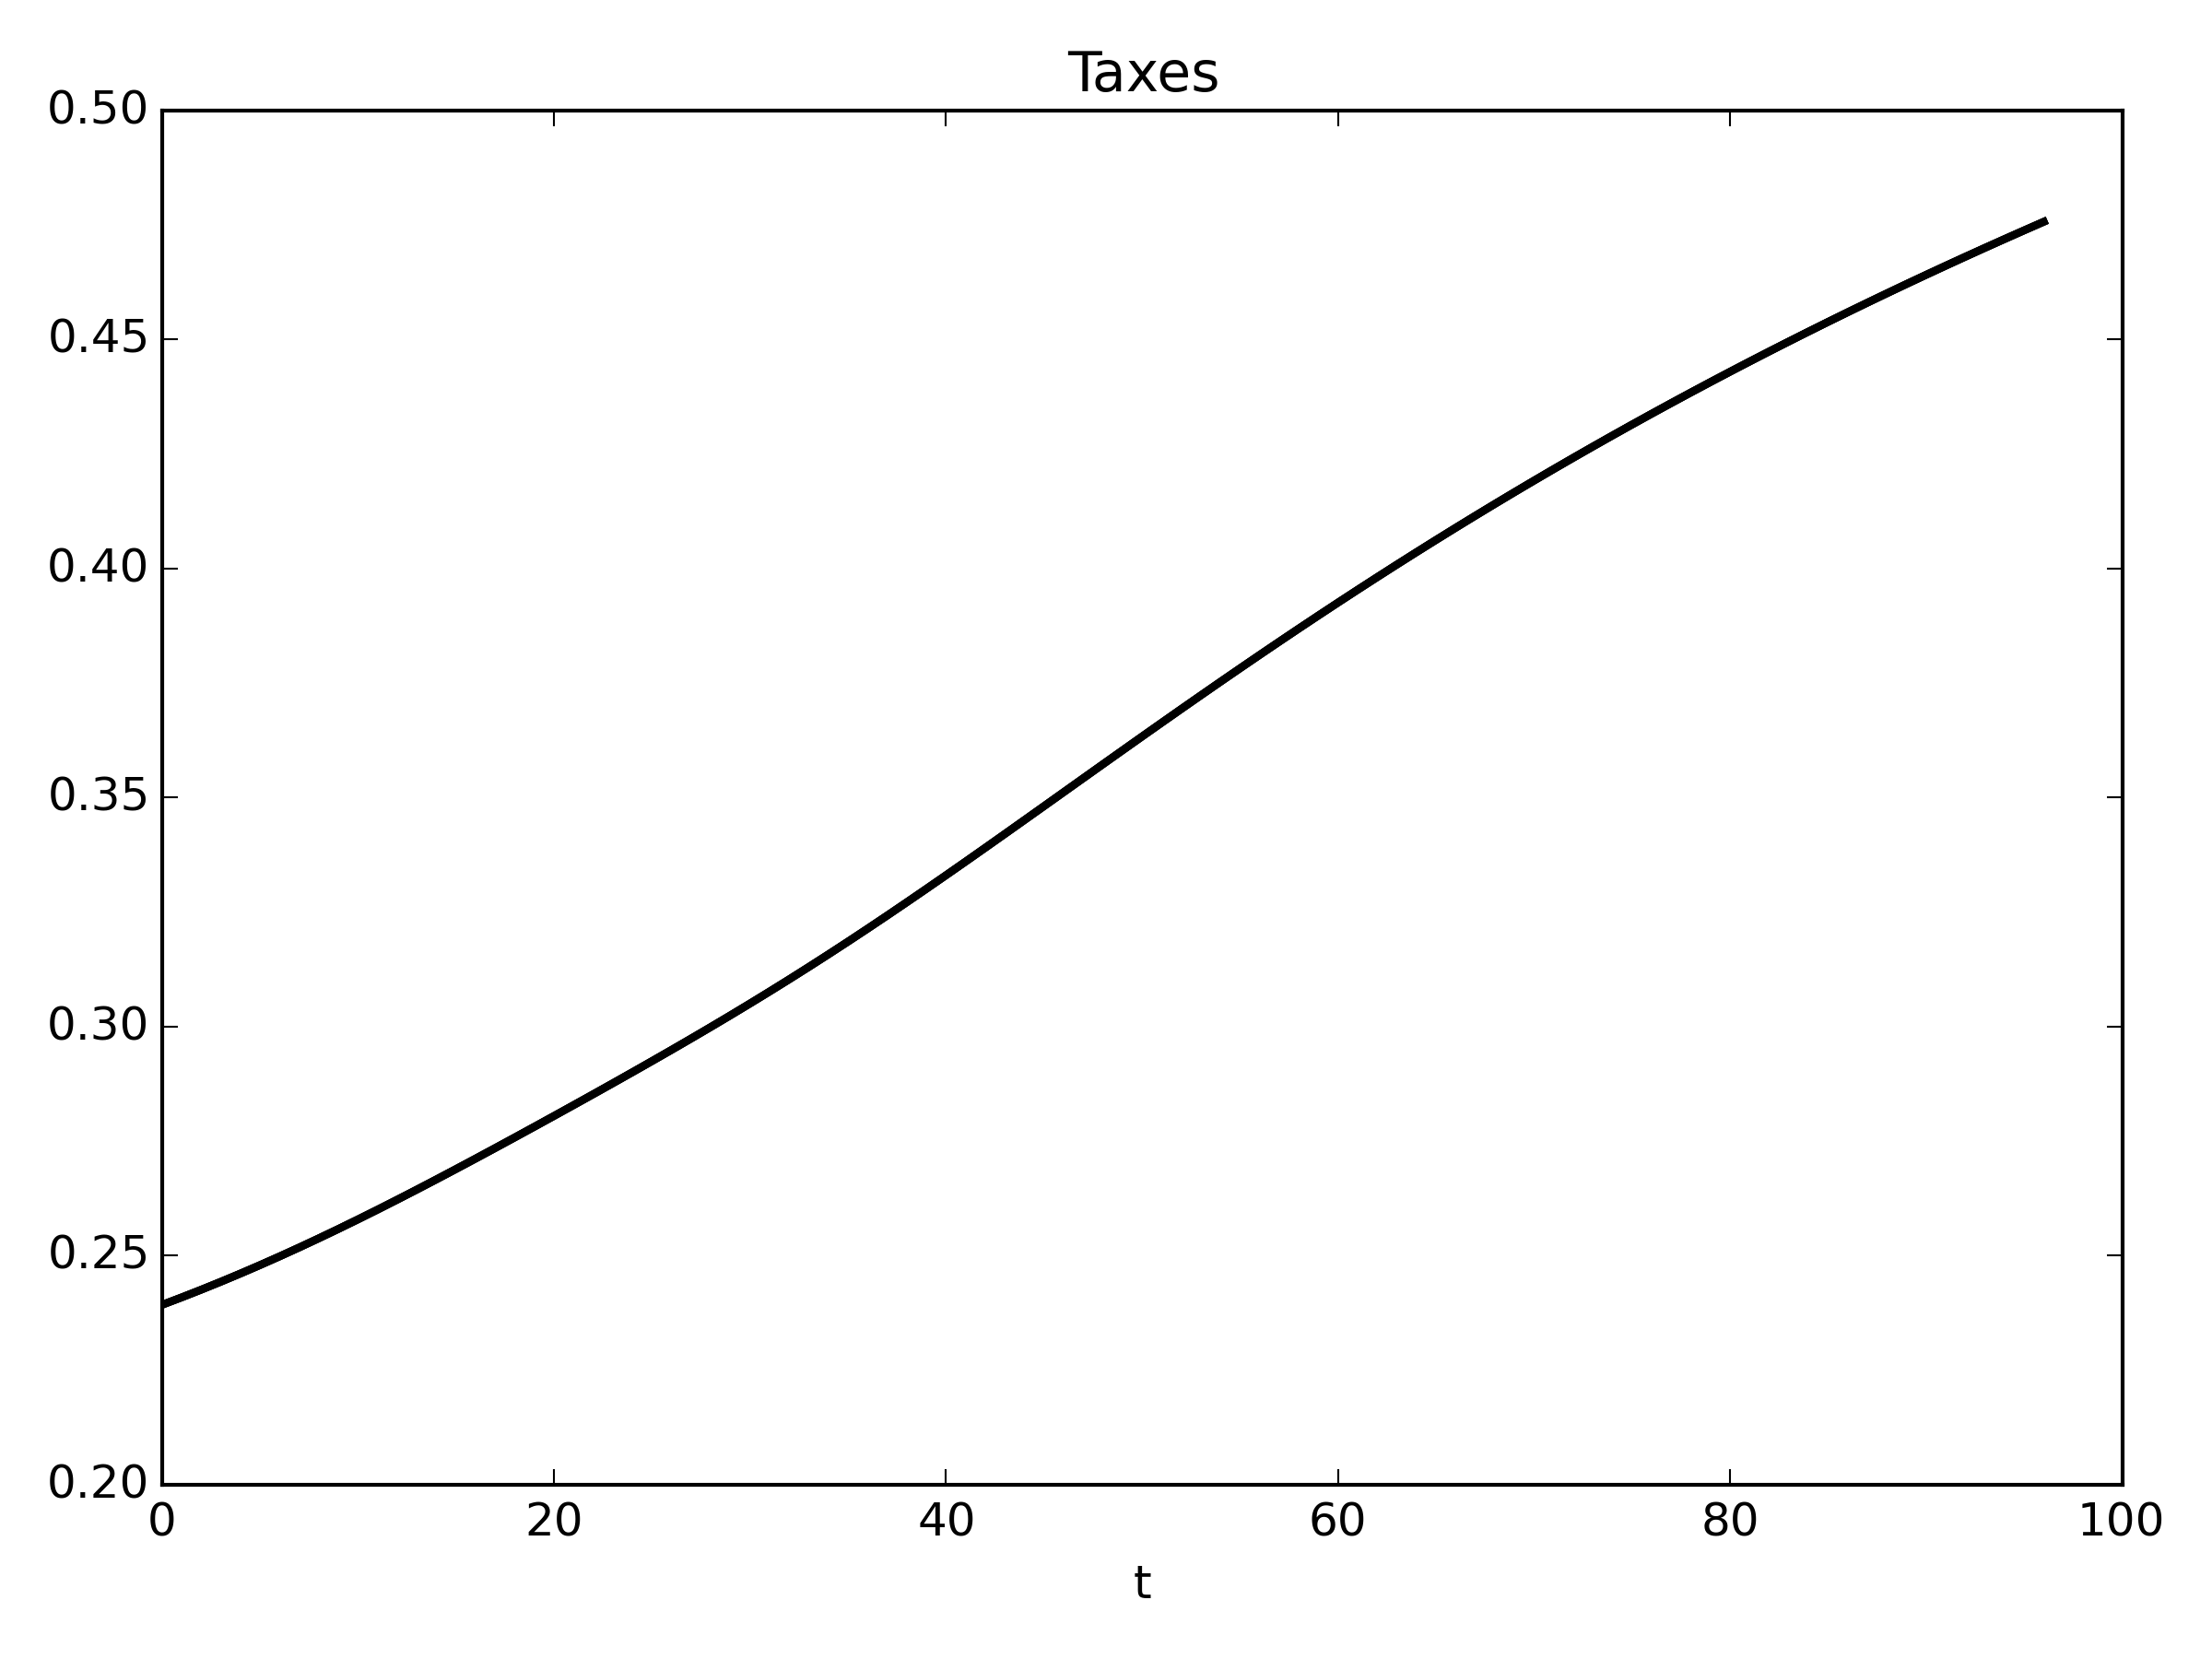
\includegraphics[width = 0.9\textwidth]{cesplots/taxes_only_bad_shocks.png}
    \caption{Tax rate for a sequence of -1 s.d shocks to aggregate productivity}
  \end{figure}

} 
 
\end{frame}


\begin{frame}
\frametitle{Short run}
Let us denote consecutive period of negative (positive) one s.d $\epsilon$ shocks a ``recession'' (boom)

\begin{itemize}
\item Engineer a recession of four periods from $t=3$. Before and after this recession, the economy receives $\epsilon_t=0$.
 
 \item Decompose responses into TFP component and inequality component:
  
 \vspace{3mm}
\centering  \textbf{Baseline:} $\log \theta_i=\epsilon [1+(.9-d(i))m]$
 \vspace{3mm}
 \begin{itemize}
  \item Only TFP: \[\log \theta_i=\epsilon\]
  \item Only Ineq: \[\log \theta_i=\epsilon [(.9-d(i))m]\]
\end{itemize}

\end{itemize}
 
\end{frame}


\begin{frame}
\frametitle{Recessions with higher inequality}
{
  \begin{figure}
    \centering
    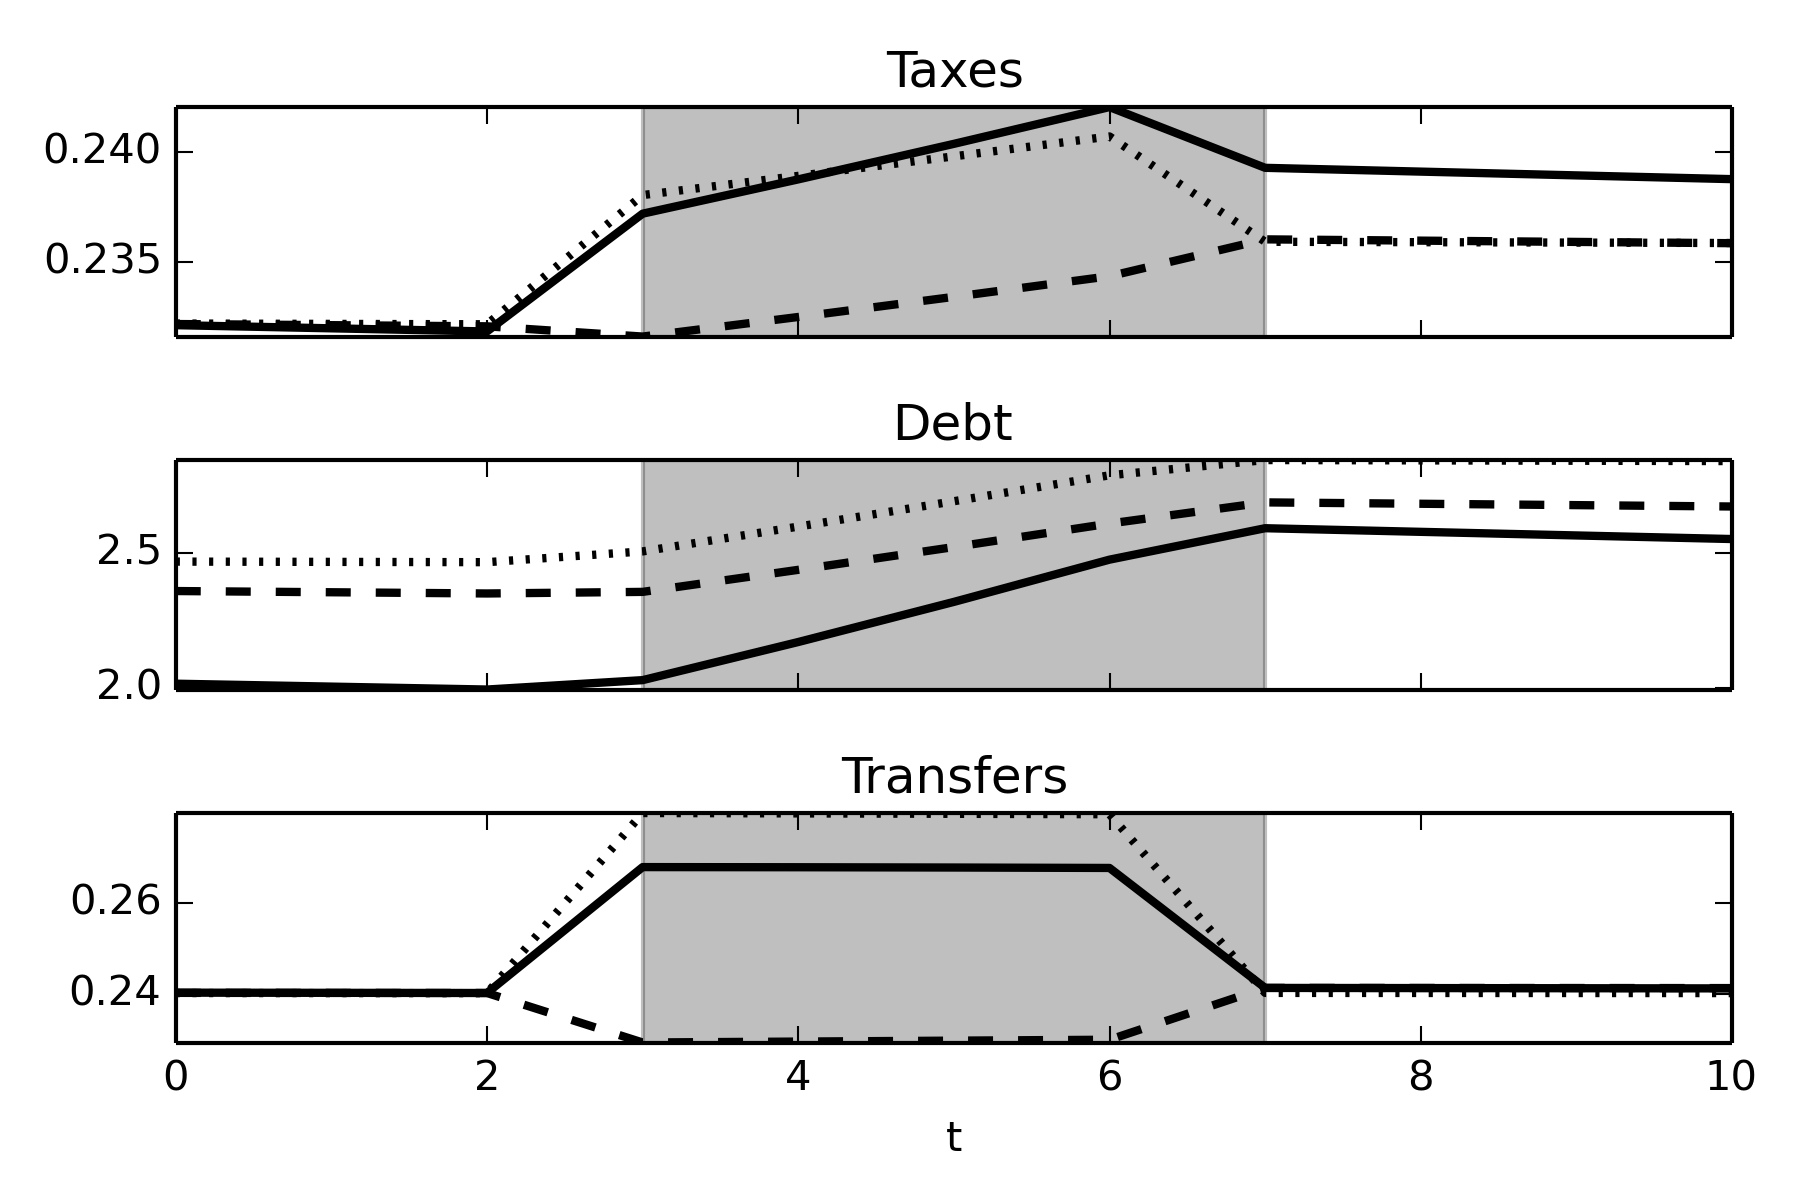
\includegraphics[width = 0.9\textwidth]{cesplots/irf_bm_chi_shocks.png}
    \caption{The bold line is the total response. The dashed (dotted) line reflects the only TFP (inequality) effect. The shaded region is the recession}
  \end{figure}

} 
\end{frame}





\begin{frame}
\frametitle{Tfp and Tfp+Ineq recessions: Sample moments}
\begin{table}[htp]
\small
\begin{tabular}{|l|l|l|}
\hline
Moments &Tfp& Tfp+Ineq\\\hline
vol. of tax rates & 0.003&0.006\\
vol. of transfers &0.01 &0.02\\
autocorr. in tax rates& 0.93&0.66\\
autocorr. in transfers& 0.17&0.18\\
corr. of taxes with tfp &0.15 &-0.63\\
corr. of transfers with tfp & 0.99&-0.98\\ \hline
\end{tabular}
\caption{These are sample moments averaged acrosss simulations of 100 periods}
\label{tab:corr}
\end{table}

\end{frame}



\begin{frame}
\frametitle{Conclusion}

\begin{itemize}
\item Size of government debt alone is not informative $\Longrightarrow $
need to know the net distribution of assets in the economy

\item Ignoring heterogeneity produces misleading results about size and
direction of the optimal policy response

\item The better ability we have to tax assets, the less debt matters and
can approximate complete markets closer
\end{itemize}


\end{frame}

\begin{frame}\label{credit limits}
\frametitle{Credit limits}
Impose $b_{i,t}\geq \underline{b}_i.$ and extend the definition of competitive eqb. in the obvious way. Now we have

\begin{theorem}
\label{thm:borrowing_constraint}  Given an initial asset distribution $\left(
\left\{ b_{i,-1}\right\} _{i},B_{-1}\right)$, let $\left\{ c_{i,t},l_{i,t}\right\} _{i,t}$ and $\left\{ R_{t}\right\}_t $ be a competitive
equilibrium allocation and interest rate sequence in an economy without
exogenous borrowing constraints. Then for any exogenous
constraints $\left\{ \underline{b}_{i}\right\} _{i}$, there is a government
tax policy $\left\{ \tau _{t},T_{t}\right\} _{t}$ such that $\left\{
c_{i,t},l_{i,t}\right\} _{i,t}$ is a competitive equilibrium
allocation in an economy with exogenous borrowing constraints $\left(
\left\{ b_{i,-1},\underline{b}_{i}\right\} _{i},B_{-1}\right) $ and $\left\{
\tau _{t},T_{t}\right\} _{t}.$
\end{theorem}
\hyperlink{ricardian eqv}{\beamerbutton{back}}

\end{frame}

\begin{frame}\label{linear appendix}
\frametitle{Ergodic distribution: Linear approximation}
\begin{itemize}
\item For a given $P(s),g(s)$, we can compress the equilibrium conditions to two functions $b(\mu\_)$ and a law of motion $\mu(s|\mu\_)$
\item Instead of approximating near a deterministic steady state we,

\begin{itemize}
\item explicitly recognize that policy rules depend on payoffs: $\mu(s|\mu\_,\{P(s)\}_s)$ and $b(\mu\_,\{P(s)\}_s)$
\item take the first order expansion with respect to both $\mu\_$ and $\{P(s)\}$ 
around the vector $(\bar{\mu},\{\bar{P}(s)\}_s)$ where $\bar{P}(s) \in \mathcal{P}^*$: 
\end{itemize}

\item The choice of $\bar P(s)$ is pinned down by 
\[
\min_{\tilde{P}\in \mathcal{P}^*} \sum_{s}\pi(s)( P(s)-\tilde{P}(s))^2.
\]
\item The law of motion approximated by
\[\mu_t-\mu^*=(\mu_{t-1}-\mu^*) B(s_t)+C(s_t)\]
\end{itemize}
\hyperlink{linearization}{\beamerbutton{back}}

\end{frame}


\begin{frame}\label{risk aversion annex}
\frametitle{More details on cases with risk aversion}
\begin{itemize}
\item With risk aversion $\|S\|=2$ is  necessary for a steady state to exist
\item Existence: Consider an economy consisting of  two types of households with only one productive agent and i.i.d binary shocks to his productivity
\small
\begin{theorem}
\label{thm long run forces}Suppose $u(c,l)=\ln c-\frac{1}{2}%
l^{2}$ and $g<\theta (s)$ for all $%
s.$ Let $x=U^2_c(s)\left[b_2(s)-b_1(s)\right]$

\begin{enumerate}
\item \textbf{Countercyclical interest rates.} If $P \left( s_{H}\right) =P\left( s_{L}\right)$, then
there exists a steady state $\left( x^{SS},\rho ^{SS}\right) $ such that $%
x^{SS}>0,\ R^{SS}\left( s_{H}\right) <R^{SS}\left( s_{L}\right) .$
\item \textbf{Procyclical interest rates.} There exists a pair  $\left\{ P \left( s_{H}\right) ,P\left( s_{L}\right)
\right\} $ such that there exists a steady state with $x^{SS}<0$ and  $R^{SS}\left( s_{H}\right) >R^{SS}\left( s_{L}\right) .$
\end{enumerate}
In both cases, tax rates $\tau(s)=\tau^{SS}$ and ratio of consumption $\frac{c_1}{c_2}$ are independent of the realized state.
\end{theorem}
\item We then develop a test for local stability as in the quasilinear case. \hyperlink{risk aversion}{\beamerbutton{back}}

\end{itemize}

\end{frame}





\begin{frame}

\frametitle{Ramsey problem: Recursive formulation}

Split  into two parts

\begin{enumerate}

\item $\mathbf{t\geq1}$: Ex-ante continuation problem with state variables $(\bm{x},\bm{\rho},s\_)$
\[\bm{x}= \beta^{-1}\left( U_{c,t-1}^{2}\tilde{b}_{2,t-1},...,U_{c,t-1}^{I}\tilde{b}_{I,t-1}\right)\]
\[ \bm{\rho }=\left( U_{c,t-1}^{2}/U_{c,t-1}^{1},...,U_{c,t-1}^{I}/U_{c,t-1}^{1}\right) \]
\item $\mathbf{t=0} $: Ex-post initial problem with state variables $(\bm{\tilde{b}_{-1}},s_{0})$
\end{enumerate}

\end{frame}


\begin{frame}
 \frametitle{Bellman Equation for  $t\geq1$}
 \scriptsize
 \begin{equation*}
V(\bm{x},\bm{\rho },s\_)=\max_{c_{i}(s),l_{i}(s),x^{\prime}(s),\rho^{\prime}(s)}
\sum_{s}\Pr (s|s\_)\left( \left[
\sum_{i}{\pi _{i}\alpha _{i}U^{i}(s)}\right] +\beta V(\bm{x}^{\prime
}(s),\bm{\rho }^{\prime }(s),s)\right)
\end{equation*}%

where the maximization is subject to
\begin{subequations}
\begin{equation*}
U_{c}^{i}(s)\left[c_{i}(s)-c_{1}(s)\right] +U_{c}^{i}(s) \left( \frac{{U_{l}^{i}(s)}}{U^i_c(s)}%
l_{i}(s)-\frac{U_{l}^{1}(s)}{U_{c}^{1}(s)}l_{1}(s)\right)+\beta x_{i}^{\prime }(s)=\frac{\color{red}x_i\color{black}P(s|s\_)U_{c}^{i}(s)}{%
 \mathbb{E}_{s\_}\bm{U}_{c}^{i}}\text{ for all }s,i\geq 2  \label{eq:BM2_Imp_cons}
\end{equation*}%
\begin{equation*}
\frac{\mathbb{E}_{s\_}P\bm{U}_{c}^{i}}{\mathbb{E}_{s\_}P\bm{U}_{c}^{1}}%
= \color{red}\rho_i\color{black}\text{ for all }i\geq 2 \label{eq:BM2_Bonds_cons}
\end{equation*}%
\begin{equation*}
\frac{U_{l}^{i}(s)}{\theta _{i}(s)U_{c}^{i}(s)}=\frac{U_{l}^{1}(s)}{\theta
_{1}(s)U_{c}^{1}(s)}\text{ for all }s,i\geq 2  \label{eq:BM2_Wages_cons}
\end{equation*}%
\begin{equation*}
\sum_{i}n_{i}c_{i}(s)+g(s)=\sum_{i}n_{i}\theta _{i}(s)l_{i}(s)  \ \ \forall s
\label{eq:BM2_Res_cons}
\end{equation*}%
\begin{equation*}
\rho _{i}^{\prime }(s)=\frac{U_{c}^{i}(s)}{U_{c}^{1}(s)} \text{ for all } s,i\geq 2 \label{eq:BM2_rhoprime}
\end{equation*}
\begin{equation*}
\underline{x}_i(s;\bm{x},\bm{\rho},s\_)\leq x_i(s)\leq \bar{x}_i(s;\bm{x},\bm{\rho},s\_)
\end{equation*}
\end{subequations}

\end{frame}



\begin{frame}
\frametitle{Bellman equation for $t=0$}
\scriptsize
 \begin{equation*}
V_0\left(\{\tilde{b}_{i,-1}\}^{I}_{i=2}, s_0\right) = \max_{c_{i,0},l_{i,0},x_0,\rho_0} {\sum_{i}\pi_i\alpha_i U^i(c_{i,0},l_{i,0}) + \beta V\left(x_0,\rho_0,s_0\right)}
\end{equation*}
where the maximization is subject to
%\textcolor{red}{XXXXX Should  a similar change to the one David recommended be executed here?}
\begin{subequations}

\begin{equation*}
U_{c,0}^{i}\left[ c_{i,0}-c_{1,0}\right] +U_{c,0}^{i} \left( \frac{U_{l,0}^{i}}{U_{c,0}^{i}} l_{i,0}-\frac{U_{l,0}^{1}}{U_{c,0}^{1}}l_{1,0}\right) +\beta x_{i,0}= U_{c,0}^{i}\tilde{b}_{i,-1}P(s_0) \text{ for all } i\geq 2
\end{equation*}

\begin{equation*}
\frac{U_{l,0}^{i}}{\theta _{i,0}U_{c,0}^{i}}=\frac{U_{l,0}^{1}}{\theta
_{1,0}U_{c}^{1,0}}\text{ for all } i\geq 2
\end{equation*}
\begin{equation*}
\sum_{i}{n_{i}c_{i,0}}+g_0=\sum_{i}{n_{i}\theta_{i,0}l_{i,0} }
\end{equation*}
\begin{equation*}
\rho _{i,0}=\frac{U_{c,0}^{i}}{U_{c,0}^{1}} \text{ for all } i\geq 2
\end{equation*}
\end{subequations}

\end{frame}
\end{document}